\begin{figure}[H]
    \centering
    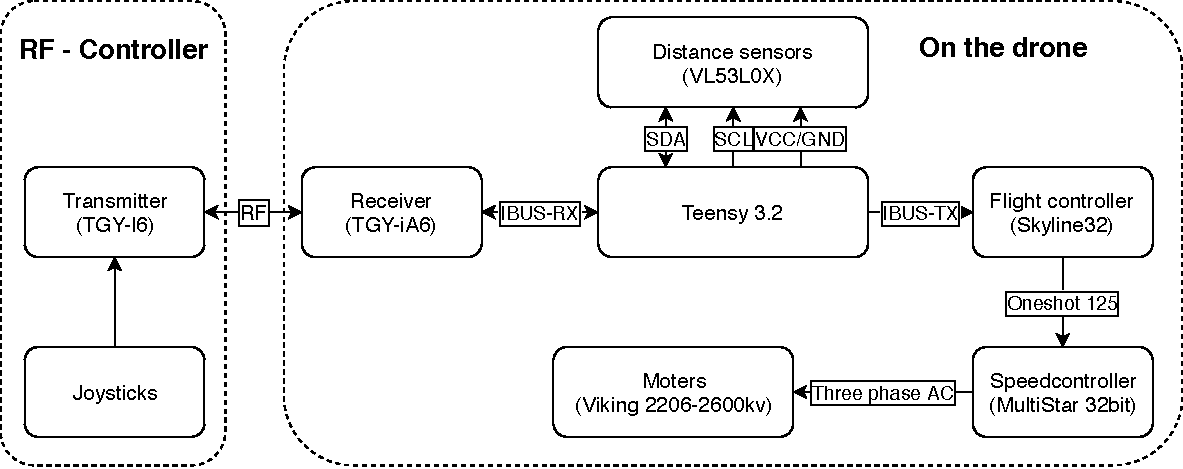
\includegraphics[width=\textwidth]{figures/ch_design/Block-diagram.pdf}
    \caption{Block diagram of how the drone works with the sensors.}
    \label{fig:block_diagram}
\end{figure}

The control diagram consists of a controller part and a drone part. As it can be seen on the system on figure \ref{fig:block_diagram}, the drone will be controlled by a RF controller using a transmitter. The transmitter communicates with the receiver on the drone by RF communication. The desired position received by the receiver will be compared with the measured data from the distance sensors. If necessary the output will be adjusted first or it will be sent to the flight controller directly. This entirely process in drone part is handled by an Teensy 3.2. The flight controller then controls the motor speed, by requesting the desired speed from the ESCs. The different blocks and communications will be described in detail in the following chapters. 